
\section{Feral Mechanisms in Rails}
\label{sec:rails-cc}

As we discussed in Section~\ref{sec:motivation}, Rails services user
requests entirely independently, with the database acting as a point
of rendezvous for concurrent operations. Given Rails's design goals of
maintaining application logic at the user level, this appears---on its
face---a somewhat cavalier proposition with respect to application
integrity. In response, Rails has developed a range of
concurrency control strategies that largely operate external to the
database and at the application level, which we term \textit{feral
  concurrency control}.

In this section, we outline four major mechanisms for guarding against
correctness anomalies under concurrent execution in Rails. We
subsequently begin our study of 67 open source applications to
determine which of these mechanisms are used in practice. In the following
section, we will determine which are are sufficient to maintain
correct data---and when they are not.

\subsection{Rails Concurrency Control Mechanisms}

Rails contains four main mechanisms for concurrency control.

\begin{myenumerate}
\item Rails provides support for \textbf{transactions}. By wrapping a
sequence of operations within a special \texttt{transaction} block,
Rails operations will execute transactionally, backed by an actual
database transaction. The database transaction either runs at the
database's configured default isolation level or, as of Rails 4.0.0, can
be configured on a per-transaction
basis~\cite{code-transaction-isolation}.

\item Rails provides support for both optimistic and pessimistic
\textbf{locking}. Applications invoke pessimistic locks on an Active
Record object by calling its \texttt{lock} method, which invokes a
\texttt{SELECT FOR UPDATE} statement in the database. Optimistic
locking is invoked by declaring a special \texttt{lock\_version} field
in an Active Record model. When a Rails process performs an update to
an optimistically locked Model, Active Record atomically checks that an object's
\texttt{lock\_version} has not changed since the process last read the
object and, if it has not changed, increments \texttt{lock\_version}
and saves the object.

\item Rails provides support for application-level
  \textbf{validations}. Each Model has a set of zero or more
  validations, or boolean-valued functions that should be run before
  the object is actually saved to the database. A model instance many
  only be saved to the database if all of its declared validations
  return true. These validations ensure, for example, that particular
  fields within a record are not null or, alternatively, are unique
  within the database. Rails provides a number of built-in validators
  but also allows arbitrary user-defined validations (we discuss
  actual validations further in subsequent sections). Each validation
  declared for a given model is run sequentially within a
  database-backed transaction upon model save.\footnote{The practice
    of wrapping validations in a transaction dates to the earliest
    Rails commit (albeit, in 2004, transactions were supported via a
    per-Ruby VM global lock~\cite{code-txn-lock}). However,
    as late as 2010, updates were only partially protected by
    transactions~\cite{code-txn-update}.}.\\[-2mm]

In contrast with the prior two mechanisms, Rails validations are a
prominent feature of the Active Record model (i.e., neither
transactions nor locks are actually discussed in the official ``Rails
Guides''). Per the Rails documentation~\cite{rails-guide}, validations ``are database
agnostic, cannot be bypassed by end users, and are convenient to test
and maintain.'' In contrast, ``[d]atabase constraints and/or stored procedures make the
validation mechanisms database-dependent and can make testing and
maintenance more difficult.'' As we will see in the next subsection,
validations are widely used by many actual applications.

\item Rails provides support for application-level
\textbf{associations}. Like validations, associations are a core
concept of the Active Record model. As the name suggests, ``an
association is a connection between two Active Record models,''
effectively acting like a foreign key in a traditional
database. Associations can be declared on one or both sides of a
one-to-one or one-to-many relationship, including transitive
dependencies (via a \texttt{:through} annotation). Declaring an
association (e.g., \texttt{:belongs\_to dept}) produces a special field
for the associated record ID within the model (e.g.,
\texttt{dept\_id}). Coupling an association with an appropriate
validation (e.g., \texttt{:presence}) ensures that the association is
indeed valid (and is, via the validation, backed by a database
transaction). Rails does not natively provide support for
database-backed foreign key constraints.
\end{myenumerate}

Overall, these four mechanisms provide a range of options for
developers. The first is squarely in the realm of traditional
concurrency control. In many cases, the latter two are reminiscent of
common database features such as referential integrity
constraints. However, others, such as UDF-based validations, are
reminiscent of proposals for more exotic, semantic-based concurrency
control primitives. We call these latter two \textit{feral} strategies
for concurrency control. As we will show shortly, the latter two
dominate in terms of developer popularity.

\subsection{Adoption in Practice}

To understand exactly how users were interacting with these
concurrency control mechanisms and determine which deserved more
study, we examined their usage in a portfolio of publicly available
open source applications.

\minihead{Application corpus} We selected 67 open source applications
built using Ruby on Rails and Active Record, representing a variety of
application domains, including eCommerce, customer relationship
management, retail point of sale, conference management, content
management, build management, project management, personal task
tracking, community management and forums, commenting, calendaring,
file sharing, Git hosting, link aggregation, crowdfunding, social
networking, and blogging. We sought projects with substantial
code-bases (average: 26,380 lines of Ruby) multiple contributors
(average: 69.2), and relative popularity (measured according to GitHub
stars) on the site. Table~\ref{table:app-summary} provides an
overview.


\begin{table*}
\scriptsize
\begin{tabular}{{|l}*{12}{l}{l|}}\hline
Name & Description & Authors & LoC Ruby & Commits &
 M & {\scriptsize T} & \scriptsize{PL} & \scriptsize{OL} & \scriptsize{V} &
 \scriptsize{A} & \scriptsize{Stars} &  \tiny{Githash} & \tiny{Last
   commit}\\\hline

Canvas LMS & {\scriptsize{Education}} & 132 & 308,113 & 12,889 & 161 & 46 & 12 & 1 & 354 & 839 & 1,251 & {\tiny\texttt{3fb8e69}} & {\tiny{10/16/14}}\\
OpenCongress & {\scriptsize{Congress data}} & 15 & 30,040 & 1,884 & 106 & 1 & 0 & 0 & 48 & 357 & 124 & {\tiny\texttt{850b602}} & {\tiny{02/11/13}}\\
Fedena & {\scriptsize{Education management}} & 4 & 48,359 & 1,471 & 104 & 5 & 0 & 0 & 153 & 317 & 262 & {\tiny\texttt{40cafe3}} & {\tiny{01/23/13}}\\
Discourse & {\scriptsize{Community discussion}} & 440 & 71,338 & 11,502 & 77 & 41 & 0 & 0 & 83 & 268 & 12,233 & {\tiny\texttt{1cf4a0d}} & {\tiny{10/20/14}}\\
Spree & {\scriptsize{eCommerce}} & 677 & 46,976 & 14,107 & 72 & 6 & 0 & 0 & 92 & 252 & 5,582 & {\tiny\texttt{aa34b3a}} & {\tiny{10/16/14}}\\
Sharetribe & {\scriptsize{Content management}} & 35 & 30,357 & 7,140 & 68 & 0 & 0 & 0 & 112 & 202 & 127 & {\tiny\texttt{8e0d382}} & {\tiny{10/21/14}}\\
ROR Ecommerce & {\scriptsize{eCommerce}} & 19 & 16,732 & 1,604 & 63 & 2 & 3 & 0 & 219 & 207 & 857 & {\tiny\texttt{c60a675}} & {\tiny{10/09/14}}\\
Diaspora & {\scriptsize{Social network}} & 388 & 31,361 & 14,640 & 63 & 2 & 0 & 0 & 66 & 128 & 9,571 & {\tiny\texttt{1913397}} & {\tiny{10/03/14}}\\
Redmine & {\scriptsize{Project management}} & 10 & 79,483 & 11,049 & 62 & 11 & 0 & 1 & 131 & 157 & 2,264 & {\tiny\texttt{e23d4d9}} & {\tiny{10/19/14}}\\
ChiliProject & {\scriptsize{Project management}} & 53 & 64,512 & 5,532 & 61 & 7 & 0 & 1 & 118 & 130 & 623 & {\tiny\texttt{984c9ff}} & {\tiny{08/13/13}}\\
Spot.us & {\scriptsize{Community reporting}} & 46 & 92,737 & 9,280 & 58 & 0 & 0 & 0 & 96 & 165 & 343 & {\tiny\texttt{61b65b6}} & {\tiny{12/02/13}}\\
Jobsworth & {\scriptsize{Project management}} & 46 & 24,469 & 7,890 & 55 & 10 & 0 & 0 & 86 & 225 & 478 & {\tiny\texttt{3a1f8e1}} & {\tiny{09/12/14}}\\
OpenProject & {\scriptsize{Project management}} & 63 & 82,764 & 11,185 & 49 & 8 & 1 & 3 & 136 & 227 & 371 & {\tiny\texttt{c1e66af}} & {\tiny{11/21/13}}\\
Danbooru & {\scriptsize{Image board}} & 25 & 27,812 & 3,738 & 47 & 9 & 0 & 0 & 71 & 114 & 238 & {\tiny\texttt{c082ed1}} & {\tiny{10/17/14}}\\
Salor Retail & {\scriptsize{Point of Sale}} & 26 & 18,007 & 2,259 & 44 & 0 & 0 & 0 & 81 & 309 & 24 & {\tiny\texttt{00e1839}} & {\tiny{10/07/14}}\\
Zena & {\scriptsize{Content management}} & 7 & 55,694 & 2,514 & 44 & 1 & 0 & 0 & 12 & 43 & 172 & {\tiny\texttt{79576ac}} & {\tiny{08/18/14}}\\
Skyline CMS & {\scriptsize{Content management}} & 7 & 10,241 & 894 & 40 & 5 & 0 & 0 & 28 & 89 & 127 & {\tiny\texttt{64b0932}} & {\tiny{12/09/13}}\\
Opal & {\scriptsize{Project management}} & 6 & 10,643 & 474 & 38 & 3 & 0 & 0 & 42 & 96 & 45 & {\tiny\texttt{11edf34}} & {\tiny{01/09/13}}\\
OneBody & {\scriptsize{Church portal}} & 33 & 19,867 & 3,976 & 36 & 3 & 0 & 0 & 97 & 140 & 1,041 & {\tiny\texttt{2dfbd4d}} & {\tiny{10/19/14}}\\
CommunityEngine & {\scriptsize{Social networking}} & 67 & 13,796 & 1,613 & 35 & 3 & 0 & 0 & 92 & 101 & 1,073 & {\tiny\texttt{a4d3ea2}} & {\tiny{10/16/14}}\\
Publify & {\scriptsize{Blogging}} & 93 & 16,555 & 5,067 & 35 & 7 & 0 & 0 & 33 & 50 & 1,274 & {\tiny\texttt{4acf86e}} & {\tiny{10/20/14}}\\
Comas & {\scriptsize{Conference management}} & 5 & 6,893 & 435 & 33 & 6 & 0 & 0 & 80 & 45 & 21 & {\tiny\texttt{81c25a4}} & {\tiny{09/09/14}}\\
BrowserCMS & {\scriptsize{Content management}} & 56 & 21,011 & 2,503 & 32 & 4 & 0 & 0 & 47 & 77 & 1,183 & {\tiny\texttt{d654557}} & {\tiny{09/30/14}}\\
RailsCollab & {\scriptsize{Project managment}} & 25 & 8,799 & 865 & 29 & 6 & 0 & 0 & 40 & 122 & 262 & {\tiny\texttt{9f6c8c1}} & {\tiny{02/16/12}}\\
Insoshi & {\scriptsize{Social network}} & 16 & 118,619 & 1,321 & 28 & 2 & 0 & 0 & 63 & 164 & 1,583 & {\tiny\texttt{9976cfe}} & {\tiny{02/24/10}}\\
OpenGovernment & {\scriptsize{Government data}} & 15 & 8,906 & 2,231 & 28 & 4 & 0 & 0 & 22 & 141 & 160 & {\tiny\texttt{fa80204}} & {\tiny{11/21/13}}\\
Tracks & {\scriptsize{Personal productivity}} & 89 & 17,312 & 3,121 & 27 & 2 & 0 & 0 & 24 & 43 & 639 & {\tiny\texttt{eb2650c}} & {\tiny{10/02/14}}\\
GitLab & {\scriptsize{Code management}} & 672 & 37,671 & 12,319 & 24 & 15 & 0 & 0 & 131 & 114 & 14,129 & {\tiny\texttt{72abe9f}} & {\tiny{10/20/14}}\\
Brevidy & {\scriptsize{Video sharing}} & 2 & 7,118 & 6 & 24 & 1 & 0 & 0 & 74 & 56 & 167 & {\tiny\texttt{d0ddb1a}} & {\tiny{01/18/14}}\\
Alchemy & {\scriptsize{Content management}} & 34 & 19,097 & 4,222 & 23 & 2 & 0 & 0 & 37 & 40 & 240 & {\tiny\texttt{91d9d08}} & {\tiny{10/20/14}}\\
Teambox & {\scriptsize{Project management}} & 48 & 32,252 & 3,155 & 22 & 2 & 0 & 0 & 56 & 116 & 1,864 & {\tiny\texttt{62a8b02}} & {\tiny{09/20/11}}\\
Fat Free CRM & {\scriptsize{Customer relationship}} & 99 & 20,754 & 4,144 & 21 & 3 & 0 & 0 & 39 & 92 & 2,384 & {\tiny\texttt{3dd2c62}} & {\tiny{10/17/14}}\\
linuxfr.org & {\scriptsize{FLOSS community}} & 29 & 8,060 & 2,271 & 20 & 1 & 0 & 0 & 50 & 50 & 86 & {\tiny\texttt{5d4d6df}} & {\tiny{10/14/14}}\\
Squash & {\scriptsize{Bug reporting}} & 28 & 15,663 & 231 & 19 & 6 & 0 & 0 & 87 & 62 & 879 & {\tiny\texttt{c217ac1}} & {\tiny{09/15/14}}\\
Shoppe & {\scriptsize{eCommerce}} & 14 & 3,115 & 349 & 19 & 1 & 0 & 0 & 58 & 34 & 208 & {\tiny\texttt{19e60c8}} & {\tiny{10/18/14}}\\
nimbleShop & {\scriptsize{eCommerce}} & 12 & 7,513 & 1,805 & 19 & 0 & 0 & 0 & 47 & 34 & 47 & {\tiny\texttt{4254806}} & {\tiny{02/18/13}}\\
Piggybak & {\scriptsize{eCommerce}} & 16 & 2,205 & 383 & 17 & 1 & 0 & 0 & 51 & 35 & 166 & {\tiny\texttt{2bed094}} & {\tiny{09/10/14}}\\
wallgig & {\scriptsize{Wallpaper sharing}} & 6 & 5,541 & 350 & 17 & 1 & 0 & 0 & 42 & 45 & 18 & {\tiny\texttt{4424d44}} & {\tiny{03/23/14}}\\
Rucksack & {\scriptsize{Collaboration}} & 7 & 5,309 & 445 & 17 & 3 & 0 & 0 & 18 & 79 & 169 & {\tiny\texttt{59703d3}} & {\tiny{10/05/13}}\\
Calagator & {\scriptsize{Online calendar}} & 48 & 8,877 & 1,766 & 16 & 0 & 0 & 0 & 8 & 11 & 196 & {\tiny\texttt{6e5df08}} & {\tiny{10/19/14}}\\
Amahi Platform & {\scriptsize{Home media sharing}} & 15 & 6,187 & 577 & 15 & 2 & 0 & 0 & 38 & 22 & 65 & {\tiny\texttt{5101c8b}} & {\tiny{08/20/14}}\\
Sprint & {\scriptsize{Project management}} & 5 & 3,053 & 71 & 14 & 0 & 0 & 0 & 50 & 45 & 247 & {\tiny\texttt{584d887}} & {\tiny{09/17/14}}\\
Citizenry & {\scriptsize{Community directory}} & 17 & 7,939 & 512 & 13 & 0 & 0 & 0 & 12 & 45 & 138 & {\tiny\texttt{e314fe4}} & {\tiny{04/01/14}}\\
Saasy & {\scriptsize{eCommerce}} & 2 & 161,092 & 21 & 12 & 5 & 0 & 0 & 41 & 117 & 520 & {\tiny\texttt{4fe610f}} & {\tiny{08/03/09}}\\
LovdByLess & {\scriptsize{Social network}} & 17 & 29,639 & 150 & 12 & 0 & 0 & 0 & 27 & 41 & 568 & {\tiny\texttt{26e79a7}} & {\tiny{10/09/09}}\\
lobste.rs & {\scriptsize{Link sharing}} & 24 & 4,927 & 624 & 12 & 8 & 0 & 0 & 20 & 40 & 646 & {\tiny\texttt{b0b9654}} & {\tiny{10/18/14}}\\
BucketWise & {\scriptsize{Personal finance}} & 10 & 4,343 & 258 & 12 & 2 & 0 & 0 & 11 & 46 & 484 & {\tiny\texttt{5c73f2b}} & {\tiny{06/10/12}}\\
Sugar & {\scriptsize{Forum}} & 13 & 7,590 & 1,316 & 11 & 1 & 0 & 0 & 20 & 53 & 89 & {\tiny\texttt{49ca79f}} & {\tiny{10/21/14}}\\
Comfy Mexican Sofa & {\scriptsize{Content management}} & 106 & 8,831 & 1,748 & 10 & 0 & 0 & 0 & 35 & 26 & 1,523 & {\tiny\texttt{fecef0c}} & {\tiny{10/09/14}}\\
Radiant & {\scriptsize{Content management}} & 100 & 15,124 & 2,385 & 9 & 3 & 0 & 1 & 26 & 12 & 1,554 & {\tiny\texttt{0c9ef9b}} & {\tiny{10/01/14}}\\
Refinery CMS & {\scriptsize{Content management}} & 438 & 10,797 & 9,112 & 9 & 0 & 0 & 0 & 16 & 8 & 2,979 & {\tiny\texttt{f4e24ef}} & {\tiny{10/20/14}}\\
Forem & {\scriptsize{Forum}} & 106 & 4,632 & 1,409 & 9 & 0 & 0 & 0 & 10 & 29 & 1,302 & {\tiny\texttt{519f2de}} & {\tiny{08/14/14}}\\
BostonRB & {\scriptsize{Ruby community}} & 40 & 2,128 & 889 & 7 & 0 & 0 & 0 & 18 & 12 & 199 & {\tiny\texttt{05fc100}} & {\tiny{10/21/14}}\\
Inkwell & {\scriptsize{Social networking}} & 6 & 6,731 & 156 & 7 & 0 & 0 & 0 & 4 & 51 & 327 & {\tiny\texttt{d1938d3}} & {\tiny{07/15/14}}\\
Boxroom & {\scriptsize{File sharing}} & 9 & 1,924 & 368 & 6 & 0 & 0 & 0 & 18 & 12 & 218 & {\tiny\texttt{1e74e06}} & {\tiny{10/18/14}}\\
Copycopter & {\scriptsize{Copy writing}} & 9 & 2,267 & 46 & 6 & 1 & 0 & 0 & 7 & 14 & 652 & {\tiny\texttt{d3607c4}} & {\tiny{06/28/12}}\\
Enki & {\scriptsize{Blogging}} & 29 & 4,584 & 562 & 6 & 1 & 0 & 0 & 5 & 7 & 835 & {\tiny\texttt{b793d48}} & {\tiny{12/01/13}}\\
Fulcrum & {\scriptsize{Project planning}} & 46 & 3,054 & 637 & 5 & 0 & 0 & 0 & 13 & 15 & 1,335 & {\tiny\texttt{8397de2}} & {\tiny{08/20/14}}\\
GitLab CI & {\scriptsize{Continuous integration}} & 80 & 3,650 & 870 & 5 & 2 & 0 & 0 & 11 & 13 & 1,188 & {\tiny\texttt{7d51134}} & {\tiny{10/17/14}}\\
Kandan & {\scriptsize{Persistent chat}} & 56 & 1,533 & 808 & 5 & 0 & 0 & 0 & 6 & 8 & 2,249 & {\tiny\texttt{15a8aab}} & {\tiny{10/06/14}}\\
Juvia & {\scriptsize{Commenting}} & 8 & 2,280 & 202 & 4 & 3 & 0 & 0 & 11 & 8 & 937 & {\tiny\texttt{43a1c48}} & {\tiny{05/09/14}}\\
Go vs Go & {\scriptsize{Go board game}} & 2 & 2,317 & 302 & 4 & 0 & 0 & 0 & 11 & 9 & 145 & {\tiny\texttt{c8d739d}} & {\tiny{02/21/13}}\\
Adopt-a-Hydrant & {\scriptsize{Civics}} & 14 & 14,163 & 1,242 & 3 & 0 & 0 & 0 & 11 & 8 & 182 & {\tiny\texttt{5b7ea0e}} & {\tiny{10/21/14}}\\
Selfstarter & {\scriptsize{Crowdfunding}} & 23 & 574 & 127 & 3 & 0 & 0 & 0 & 1 & 4 & 2,688 & {\tiny\texttt{740075f}} & {\tiny{05/16/14}}\\
Heaven & {\scriptsize{Code deployment}} & 19 & 2,083 & 387 & 2 & 0 & 0 & 0 & 2 & 2 & 163 & {\tiny\texttt{2d4162e}} & {\tiny{10/21/14}}\\
Carter & {\scriptsize{eCommerce}} & 3 & 1,052 & 70 & 2 & 1 & 0 & 0 & 0 & 12 & 22 & {\tiny\texttt{60ad49d}} & {\tiny{07/22/14}}\\
Obtvse & {\scriptsize{Blogging}} & 27 & 427 & 393 & 1 & 0 & 0 & 0 & 3 & 0 & 1,516 & {\tiny\texttt{1542856}} & {\tiny{03/21/13}}\\\hline
\textbf{Average:} &  & \textbf{69.21} & \textbf{26,380.48} & \textbf{2,953.31} & \textbf{29.21} & \textbf{3.87} & \textbf{0.24} & \textbf{0.10} & \textbf{53.00} & \textbf{96.04} & \textbf{1,272.42} &  & {\tiny\textbf{02/06/14}}\\

\hline
\end{tabular}
\caption{Corpus of applications used in analysis. (M: Models, T:
  Transactions, PL: Pessimistic Locking, OL: Optimistic Locking, V: Validations, A: Associations)}
\label{table:app-summary}
\end{table*}

While several of these applications are projects undertaken by
hobbyists, many are either commercially supported (e.g., Canvas LMS,
Discourse, Spree, GitLab) and/or have a large open source community
(e.g., Radiant, Comfortable Mexican Sofa, Diaspora). Undoubtedly, a
larger-scale commercial, closed-source Rails projects such as Twitter,
GitHub, or Airbnb might exhibit different trends than those we observe
here. However, in the open source domain, we believe these
applications represent a diverse selection of Rails use cases.

\minihead{Mechanism usage} We performed a simple analysis of the
applications to determine how each of the concurrency control
mechanisms from each application were used (see Appendix for
methodological details).

Overwhelmingly, applications did not use transactions or locks
(Figure~\ref{fig:usages} and Table~\ref{table:app-summary}). On
average, applications used 0.13 transactions, 0.01 locks, 1.82
validations, and 3.30 associations per model (with an average of 29.1
models per application). While 46 (68.7\%) of applications at least
transactions, 66 (98.5\%) used at least one validation or
association. Only six applications (8.9\%) used locks, with
pessimistic locking over twice as common as optimistic locking.

Thus, as a general trend, we find that validations and associations
are, respectively, 14 and 25 times more common than transactions and
orders of magnitude more common than locking. The feral
mechanisms---that rely on application-enforced integrity
maintenance---are---in keeping with the Rails philosophy---favored by
these application developers. That is, rather than adopting the use of
traditional transactional updates, Rails application writers chose to
instead declaratively specify correctness criteria and have the ORM
system check the criteria for them instead. It is unclear and even
unlikely that these declarative criteria are a complete specification
of program correctness: undoubtedly, some of these programs contain
errors. However, from the perspective of database usability and
idiomatic web programming patterns, this reliance on application-level
correctness criteria hints at an alternative developer mentality than
users of traditional database concurrency control.   We
devote much of the remainder of this work to examining exactly what
these feral mechanisms are attempting preserve (and whether they are
actually correct in doing so).

Over the course of our investigation, we found a variety of
interesting anecdotes. For example, the eCommerce application Spree
uses six transactions, one for each of cancelling an order and and
approving an order (atomically setting the user ID and timestamp),
transfering shipments between fulfillment locations (e.g.,
warehouses), transferring items between shipments, transfering stock
between fulfillment locations, and updating an order's specific
inventory status. A perhaps more natural point of contention
(reminsicent of the canonical bank example from database textbooks) is
mediating access to the available stock in an inventory. Performing
delta adjustments to the available stock
(\texttt{adjust\_count\_on\_hand(value)}) is protected via a
pessimistic lock, but setting the available stock
(\texttt{set\_count\_on\_hand(value)}) is not. The stock level itself
is wrapped in a validation ensuring non-negative balances
(\texttt{validates :count\_on\_hand, numericality: {
    greater\_than\_or\_equal\_to: 0 }, if:
  :verify\_count\_on\_hand?}). At one point, Spree's inventory was
protected by an optimistic lock; it was removed due to failing
customer checkout requests. On the relevant GitHub issue, a committer
notes that ``I think we should get rid of the [optimistic lock] if
there's no documentation about why it's there...I think we can look at
this issue again in a month's time and see if there's been any
problems since you turned it off''~\cite{code-optimistic-issue}. Thus,
the choice of (and even use of) concurrency control is sometimes an
ad-hoc process.

The remainder of the corpus contains a number of such phenomena. The
use of each style of concurrency control varies across repositories,
but our results demonstrate a clear trend towards feral mechanisms
within Rails. As a consequence of the breadth of our study (and paper
formatting limitations), we are not able to discuss every application
in detail (though the source code of each and, fortunately, the Git
history and, often, issue trackers are publicly available for
inspection).

\begin{figure}
  \newcommand{\skipht}{\\[-2em]}
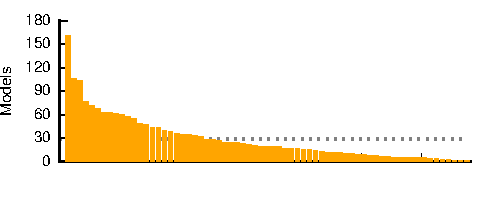
\includegraphics[width=\columnwidth]{figs/models-single-bar.pdf}\skipht
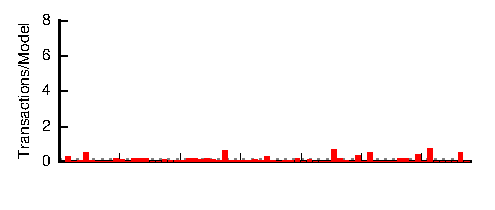
\includegraphics[width=\columnwidth]{figs/transactions-single-bar.pdf}\skipht
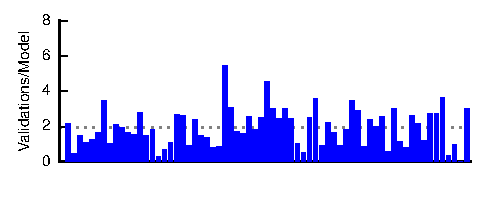
\includegraphics[width=\columnwidth]{figs/validations-single-bar.pdf}\skipht
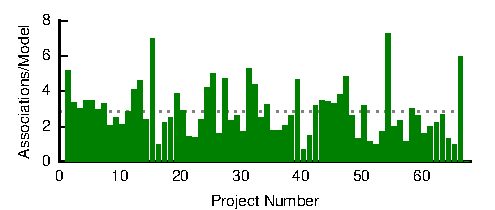
\includegraphics[width=\columnwidth]{figs/associations-single-bar.pdf}\skipht
\caption{Use of concurrency control mechanisms in Rails
  applications. Dotted line shows average for plot.}
\label{fig:usages}
\end{figure}



\minihead{Additional metrics} To better illustrate how programmers
were using each of these mechanisms, we report on two additional
analyses.

First, we analyzed the number of models, transactions, validations,
and associations over each project's lifetime. Using each
application's Git logs, we repeated the above analysis at a fixed set
of intervals through the application's history (by commits). At each
interval, we recorded the number of occurrences of each of these
constructs relative to the total number of occurences in the project
in the latest repository we examined. Figure~\ref{fig:historical}
plots the median number of occurences across all projects. Notably, by
the time 50\% of the commits have been entered into the repository,
over 75\% of the models, transactions, validations, and associations
have been written. This suggests that the Model layer may be less
volatile than the View and Controller components of the
applications. Moreover, the initial proportion of validations and
associations is higher than the initial proportion of transactions:
the data model appears to stabilize faster than the controller
logic. It is unclear whether the bulk of transaction usage is added in
order to compensate for, say, concurrency violations, or is instead
due to growth in Controller code and business logic.

\begin{figure}
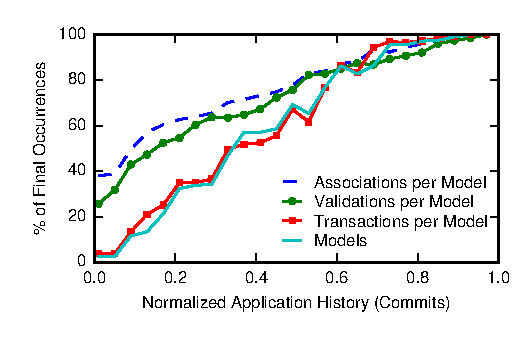
\includegraphics[width=\columnwidth]{figs/historical-median.pdf}\vspace{-2em}
\caption{Median use of Rails mechanisms over time.}
\label{fig:historical}
\end{figure}

Second, we analyze the distribution of authors to commits compared to
the distribution of authors to validations and associations
authored.\footnote{We chose to analyze commits authored rather than
  lines of code written because git tracks large-scale code
  refactoring commits as an often large set of deletions and
  insertions. Nevertheless, we observed a close correlation between
  lines of code and commits authored.} As Figure~\ref{fig:cdfs}
demonstrates, 95\% of all commits are authored by 42.4\% of
authors. However, 95\% of invariants are authored by only 20.3\% of
authors. This is reminiscent of traditional database schema
authorship, where a smaller number of authors (e.g., DBAs) modify the
schema than contribute to the actual application code.

\begin{figure}
  \newcommand{\skipht}{\\[-2em]}
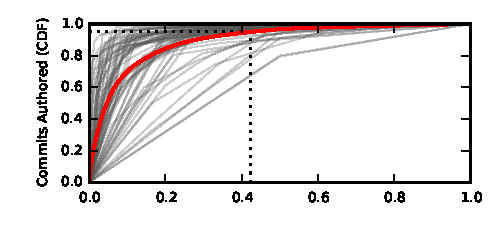
\includegraphics[width=\columnwidth]{figs/commit-authorship-cdf.pdf}\vspace{-2em}
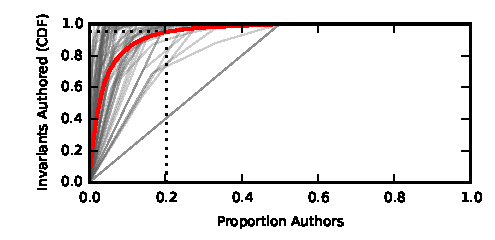
\includegraphics[width=\columnwidth]{figs/invariant-authorship-cdf.pdf}\vspace{-1em}
\caption{CDFs of authorship of invariants and commits.}
\label{fig:cdfs}
\end{figure}

\subsection{Discussion}

Returning to the Rails design philosphy, the applications we have
encountered do indeed express their logic at the application
layer. There is little actual communication of correctness critera to
the database layer. Part of this is due to limitations within
Rails. As we have mentioned, there is no way to actually declare a
foreign key constraint in Rails without importing additional
third-party modules. However, insofar as Rails is an ``opinionated''
framework encouraging an idiomatic programming style, if our
application corpus is any indication, DHH and his co-authors
advocating application-level data management appear to have succeeded en
masse.

Having observed the relative popularity of these mechanisms, we turn
our attention to the question of their correctness. Specifically, do
these application-level criteria actually enforce the constraints that
they claim to enforce? We restrict ourself to studying declared
validations and associations for three reasons. First, as we have
seen, these constructs are widely used in the codebases we have
studied, and, ostensibly, more widely used in the Rails community than
the alternatives. Second, these constructs represent a deviation from
standard concurrency control techniques and are therefore perhaps more
likely to contain errors. Third, while analyzing latent constraints (i.e.,
those that might be determined via more sophisticated techniques such
as pre- and post-condition invariant mining and/or by interviewing each
developer on each project) would be instructive, this is difficult to
scale. We view these forms of analysis as worthwhile avenues for
future research.
